\section{Convolutional Neural Networks}
\label{sec:convolutional-neural-networks}

Although neural networks can be applied to computer vision tasks, to get good generalization performance, it is beneficial to incorporate prior knowledge into the network architecture \cite{LeCun:1989}. Convolutional neural networks aim to use spatial information between the pixels of an image. Therefore, they are based on discrete convolution. After introducing discrete convolution, we discuss the basic components of convolutional neural networks as described in \cite{JarrettKavukcuogluRanzatoLeCun:2009} and \cite{LeCunKavukvuogluFarabet:2010}.

\subsection{Convolution}
\label{subsec:convolution}

For simplicity we assume a grayscale image to be defined by a function
\begin{align}
	I : \{1, \ldots, n_1\} \times \{1, \ldots, n_2\} \rightarrow W \subseteq \mathbb{R}, (i,j) \mapsto I_{i,j}
\end{align}
such that the image $I$ can be represented by an array of size $n_1 \times n_2$\footnote{Often, $W$ will be the set $\{0, \ldots, 255\}$ representing an $8$-bit channel. Then, a color image can be represented by an array of size $n_1 \times n_2 \times 3$ assuming three color channels, for example RGB.}. Given the filter $K \in \mathbb{R}^{2h_1+1 \times 2h_2+1}$, the discrete convolution of the image $I$ with filter $K$ is given by
\begin{align}
	\label{eq:convolution}
	\left(I \ast K\right)_{r,s} := \sum _{u = -h_1} ^{h_1} \sum _{v = -h_2}^{h_2} K_{u,v} I_{r+u,s+v}
\end{align}
where the filter $K$ is given by
\begin{align}
	K =
 	\begin{pmatrix}
  		K_{-h_1,-h_2} & \ldots & K_{-h_1,h_2}\\
  		\vdots & K_{0,0} & \vdots\\
  		K_{h_1,-h_2} & \ldots & K_{h_1,h_2}\\
 	\end{pmatrix}.
\end{align}
Note that the behavior of this operation towards the borders of the image needs to be defined properly\footnote{As example, consider a gray scale image of size $n_1 \times n_2$. When applying an arbitrary filter of size $2h_1+1 \times 2h_2+1$ to the pixel at location $(1,1)$ the sum of equation \eqref{eq:convolution} includes pixel locations with negative indices. To solve this problem, several approaches can be considered, as for example padding the image in some way or applying the filter only for locations where the operation is defined properly resulting in the output array being smaller than the image.}.

A commonly used filter for smoothing is the discrete Gaussian filter $K_{G(\sigma)}$ \cite{ForsythPonce:2002} which is defined by
\begin{align}
	\label{eq:gaussian-filter}
	\left(K_{G(\sigma)}\right)_{r,s} = \frac{1}{\sqrt{2\pi}\sigma^2} \exp \left(\frac{r^2 + s^2}{2\sigma^2}\right)
\end{align}
where $\sigma$ is the standard deviation of the Gaussian distribution \cite{ForsythPonce:2002}.

\subsection{Layers}

We follow \cite{JarrettKavukcuogluRanzatoLeCun:2009} and introduce the different types of layers used in convolutional neural networks. Based on these layers, complex architectures as used for classification in \cite{CiresanMeierSchmidhuber:2012} and \cite{KrizhevskySutskeverHinton:2012} can be built by stacking multiple layers. % As in \cite{JarrettKavukcuogluRanzatoLeCun:2009} we label the different types of layers to allow the easy description of complicated architectures.

\subsubsection{Convolutional Layer}

Let layer $l$ be a convolutional layer. Then, the input of layer $l$ comprises $m_1^{(l-1)}$ feature maps from the previous layer, each of size $m_2^{(l-1)} \times m_3^{(l-1)}$. In the case where $l = 1$, the input is a single image $I$ consisting of one or more channels. This way, a convolutional neural network directly accepts raw images as input. The output of layer $l$ consists of $m_1^{(l)}$ feature maps of size $m_2^{(l)} \times m_3^{(l)}$. The $i^{\text{th}}$ feature map in layer $l$, denoted $Y_i^{(l)}$, is computed as
\begin{align}
	\label{eq:convolutional-layer}
	Y_i^{(l)} = B^{(l)}_{i} + \sum _{j = 1}^{m_1^{(l-1)}} K^{(l)}_{i,j} \ast Y_j^{(l-1)}
\end{align}
where $B_i^{(l)}$ is a bias matrix and $K^{(l)}_{i,j}$ is the filter of size $2h_1^{(l)} + 1 \times 2h_2^{(l)} + 1$ connecting the $j^{\text{th}}$ feature map in layer $(l-1)$ with the $i^{\text{th}}$ feature map in layer $l$ \cite{LeCunKavukvuogluFarabet:2010}\footnote{Note the difference between a feature map $Y_i^{(l)}$ comprising $m_2^{(l)} \cdot m_3^{(l)}$ units arranged in a two-dimensional array and a single unit $y_i^{(l)}$ as used in the multilayer perceptron.}. As mentioned above, $m_2^{(l)}$ and $m_3^{(l)}$ are influenced by border effects. When applying the discrete convolution only in the so called valid region of the input feature maps, that is only for pixels where the sum of equation \eqref{eq:convolution} is defined properly, the output feature maps have size
\begin{align}
	m_2^{(l)} = m_2^{(l-1)} - 2h_1^{(l)}\quad \text{ and }\quad m_3^{(l)} = m_3^{(l-1)} - 2h_2^{(l)}.
\end{align}
Often the filters used for computing a fixed feature map $Y_i^{(l)}$ are the same, that is $K_{i,j}^{(l)} = K _{i,k}^{(l)}$ for $j \neq k$. In addition, the sum in equation \eqref{eq:convolutional-layer} may also run over a subset of the input feature maps.

To relate the convolutional layer and its operation as defined by equation \eqref{eq:convolutional-layer} to the multilayer perceptron, we rewrite the above equation. Each feature map $Y_i^{(l)}$ in layer $l$ consists of $m_2^{(l)} \cdot m_3^{(l)}$ units arranged in a two-dimensional array. The unit at position $(r,s)$ computes the output
\begin{align}
	\left(Y_i^{(l)}\right)_{r,s} &= \left(B_i^{(l)}\right)_{r,s} + \sum _{j = 1}^{m_1^{(l-1)}} \left(K^{(l)}_{i,j} \ast Y_j^{(l-1)}\right)_{r,s}\\
	&= \left(B_i^{(l)}\right)_{r,s} + \sum _{j = 1}^{m_1^{(l-1)}} \sum _{u = - h_1^{(l)}} ^{h_1^{(l)}} \sum _{v = - h_2^{(l)}} ^{h_2^{(l)}} \left(K^{(l)}_{i,j}\right)_{u,v} \left(Y_j^{(l-1)}\right)_{r+u,s+v}.
\end{align}
The trainable weights of the network can be found in the filters $K^{(l)}_{i,j}$ and the bias matrices $B_i^{(l)}$.

As we will see in section \ref{subsubsec:pooling-layer}, subsampling is used to decrease the effect of noise and distortions. As noted in \cite{CiresanMeierMasciGambardellaSchmidhuber:2011}, subsampling can be done using so called skipping factors $s_1^{(l)}$ and $s_2^{(l)}$. The basic idea is to skip a fixed number of pixels, both in horizontal and in vertical direction, before applying the filter again. With skipping factors as above, the size of the output feature maps is given by
\begin{align}
	m_2^{(l)} = \frac{m_2^{(l-1)} - 2h_1^{(l)}}{s_1^{(l)} + 1}\quad \text{ and }\quad m_3^{(l)} = \frac{m_3^{(l-1)} - 2h_2^{(l)}}{s_2^{(l)} + 1}.
\end{align}
\begin{SCfigure}[2\sidecaptionrelwidth][t]
	\centering
	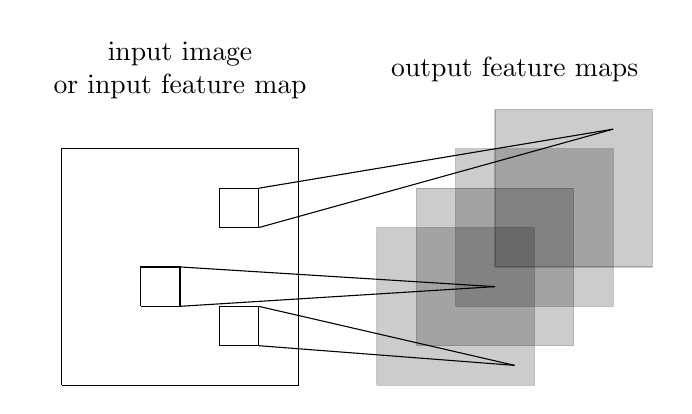
\begin{tikzpicture}
		\node at (1.5,4){\begin{tabular}{c}input image\\or input feature map\end{tabular}};
	
		\draw (0,0) -- (3,0) -- (3,3) -- (0,3) -- (0,0);
		
		\draw (2,2) -- (2.5,2) -- (2.5,2.5) -- (2,2.5) -- (2,2);
		\draw (2,0.5) -- (2.5,0.5) -- (2.5,1) -- (2,1) -- (2,0.5);
		\draw (1,1) -- (1.5,1) -- (1.5,1.5) -- (1,1.5) -- (1,1);
		
		\draw (2.5,2) -- (7,3.25);
		\draw (2.5,2.5) -- (7,3.25);

		\draw (2.5,1) -- (5.75,0.25);
		\draw (2.5,0.5) -- (5.75,0.25);
		
		\draw (1.5,1.5) -- (5.5,1.25);
		\draw (1.5,1) -- (5.5,1.25);
		
		\node at (5.75,4){\begin{tabular}{c}output feature maps\end{tabular}};
		
		\draw[fill=black,opacity=0.2,draw=black] (5.5,1.5) -- (7.5,1.5) -- (7.5,3.5) -- (5.5,3.5) -- (5.5,1.5);
		\draw[fill=black,opacity=0.2,draw=black] (5,1) -- (7,1) -- (7,3) -- (5,3) -- (5,1);
		\draw[fill=black,opacity=0.2,draw=black] (4.5,0.5) -- (6.5,0.5) -- (6.5,2.5) -- (4.5,2.5) -- (4.5,0.5);
		\draw[fill=black,opacity=0.2,draw=black] (4,0) -- (6,0) -- (6,2) -- (4,2) -- (4,0);
	\end{tikzpicture}
	\caption[Illustration of a convolutional layer.]{Illustration of a single convolutional layer. If layer $l$ is a convolutional layer, the input image (if $l = 1$) or a feature map of the previous layer is convolved by different filters to yield the output feature maps of layer $l$.}
	\label{fig:convolutional-layer}
\end{SCfigure}

\subsubsection{Non-Linearity Layer}
\label{subsubsec:rectification-layer}

If layer $l$ is a non-linearity layer, its input is given by $m_1^{(l)}$ feature maps and its output comprises again $m_1^{(l)} = m_1^{(l-1)}$ feature maps, each of size $m_2^{(l-1)} \times m_3^{(l-1)}$ such that $m_2^{(l)} = m_2^{(l-1)}$ and $m_3^{(l)} = m_3^{(l-1)}$, given by
\begin{align}
	Y_i^{(l)} = f \left(Y_i^{(l-1)}\right).
\end{align}
where $f$ is the activation function used in layer $l$ and operates point wise. In \cite{JarrettKavukcuogluRanzatoLeCun:2009} additional gain coefficients are added:
\begin{align}
	Y_i^{(l)} = g_i f\left(Y_i^{(l-1)}\right).
\end{align}

A convolutional layer including a non-linearity, with hyperbolic tangent activation functions and gain coefficients is denoted by $F_{\text{CSG}}$\footnote{C for convolutional layer, S for sigmoid/hyperbolic tangent activation functions and G for gain coefficients. In \cite{JarrettKavukcuogluRanzatoLeCun:2009} the filter size is added as subscript such that $F_{\text{CSG}}^{7 \times 7}$ denotes the usage of $7 \times 7$ filters. Additionally, the number of used filters is added as follows: $32F_{\text{CSG}}^{7 \times7}$. We omit the number of filters as we assume full connectivity such that the number of filters is given by $m_1^{(l)}\cdot m_1^{(l-1)}$.}. Note that in \cite{JarrettKavukcuogluRanzatoLeCun:2009} this constitutes a single layer whereas we separate the convolutional layer and the non-linearity layer.

\subsubsection{Rectification}

Let layer $l$ be a rectification layer. Then its input comprises $m_1^{(l-1)}$ feature maps of size $m_2^{(l-1)} \times m_3^{(l-1)}$ and the absolute value for each component of the feature maps is computed:
\begin{align}
	\label{eq:rectification}
	Y_i^{(l)} = \left|Y_i^{(l)}\right|
\end{align}
where the absolute value is computed point wise such that the output consists of $m_1^{(l)} = m_1^{(l-1)}$ feature maps unchanged in size\footnote{Note that equation \eqref{eq:rectification} can easily be applied to fully-connected layers as introduced in section \ref{subsubsec:fully-connected-layer}, as well.}. Experiments in \cite{JarrettKavukcuogluRanzatoLeCun:2009} show that rectification plays a central role in achieving good performance.

Although rectification could be included in the non-linearity layer \cite{LeCunKavukvuogluFarabet:2010}, we follow \cite{JarrettKavukcuogluRanzatoLeCun:2009} and add this operation as an independent layer. The rectification layer is denoted by $R_{\text{abs}}$.

\subsubsection{Local Contrast Normalization Layer}
\label{subsubsec:contrast-normalization}

Let layer $l$ be a contrast normalization layer. The task of a local contrast normalization layer is to enforce local competitiveness between adjacent units within a feature map and units at the same spatial location in different feature maps. We discuss subtractive normalization as well as brightness normalization. An alternative, called divisive normalization, can be found in \cite{JarrettKavukcuogluRanzatoLeCun:2009} or \cite{LeCunKavukvuogluFarabet:2010}. Given $m_1^{(l-1)}$ feature maps of size $m_2^{(l-1)} \times m_3^{(l-1)}$, the output of layer $l$ comprises $m_1^{(l)} = m_1^{(l-1)}$ feature maps unchanged in size. The subtractive normalization operation computes
\begin{align}
	Y_i^{(l)} = Y_i^{(l-1)} - \sum _{j = 1}^{m^{(l-1)}} K_{G(\sigma)} \ast Y_j^{(l-1)}
\end{align}
where $K_{G(\sigma)}$ is the Gaussian filter from equation \eqref{eq:gaussian-filter}.

In \cite{KrizhevskySutskeverHinton:2012} an alternative local normalization scheme called brightness normalization is proposed to be used in combination with rectified linear units. Then the output of layer $l$ is given by
\begin{align}
\label{eq:brightness-normalization}
	\left(Y_i^{(l)}\right)_{r,s} = \frac{\left( Y_i^{(l-1)} \right)_{r,s}}{\left(\kappa + \mu \sum _{j = 1}^{m_1^{(l-1)}} \left( Y_j^{(l-1)} \right)_{r,s}^2\right)^\mu}
\end{align}
where $\kappa$, $\lambda$, $\mu$ are hyperparameters which can be set using a validation set \cite{KrizhevskySutskeverHinton:2012}. The sum in equation \eqref{eq:brightness-normalization} may also run over a subset of to the feature maps in layer $(l-1)$. Local contrast normalization layers are denoted $N_S$ and $N_B$, respectively.

\subsubsection{Feature Pooling and Subsampling Layer}
\label{subsubsec:pooling-layer}

\begin{SCfigure}[2\sidecaptionrelwidth][t!]
	\centering
	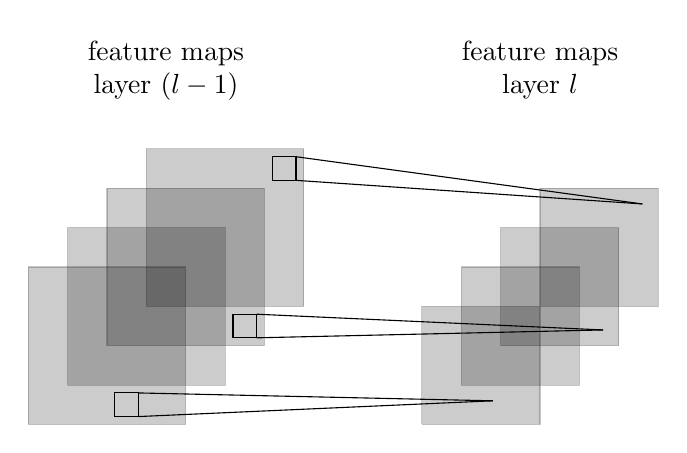
\begin{tikzpicture}
		\node at (1.75,4.5){\begin{tabular}{c}feature maps\\layer $(l-1)$\end{tabular}};
		
		\draw[fill=black,opacity=0.2,draw=black] (1.5,1.5) -- (3.5,1.5) -- (3.5,3.5) -- (1.5,3.5) -- (1.5,1.5);
		\draw[fill=black,opacity=0.2,draw=black] (1,1) -- (3,1) -- (3,3) -- (1,3) -- (1,1);
		\draw[fill=black,opacity=0.2,draw=black] (0.5,0.5) -- (2.5,0.5) -- (2.5,2.5) -- (0.5,2.5) -- (0.5,0.5);
		\draw[fill=black,opacity=0.2,draw=black] (0,0) -- (2,0) -- (2,2) -- (0,2) -- (0,0);
		
		\draw (3.1,3.1) -- (3.4,3.1) -- (3.4,3.4) -- (3.1,3.4) -- (3.1,3.1);
		\draw (2.6,1.1) -- (2.9,1.1) -- (2.9,1.4) -- (2.6,1.4) -- (2.6,1.1);
		\draw (1.1,0.1) -- (1.4,0.1) -- (1.4,0.4) -- (1.1,0.4) -- (1.1,0.1);
		
		\draw (3.4,3.4) -- (7.8,2.8);
		\draw (3.4,3.1) -- (7.8,2.8);
		
		\draw (2.9,1.4) -- (7.3,1.2);
		\draw (2.9,1.1) -- (7.3,1.2);
		
		\draw (1.4,0.4) -- (5.9,0.3);
		\draw (1.4,0.1) -- (5.9,0.3);
		
		\node at (6.5,4.5){\begin{tabular}{c}feature maps\\layer $l$\end{tabular}};
		
		\draw[fill=black,opacity=0.2,draw=black] (6.5,1.5) -- (8,1.5) -- (8,3) -- (6.5,3) -- (6.5,1.5);
		\draw[fill=black,opacity=0.2,draw=black] (6,1) -- (7.5,1) -- (7.5,2.5) -- (6,2.5) -- (6,1);
		\draw[fill=black,opacity=0.2,draw=black] (5.5,0.5) -- (7,0.5) -- (7,2) -- (5.5,2) -- (5.5,0.5);
		\draw[fill=black,opacity=0.2,draw=black] (5,0) -- (6.5,0) -- (6.5,1.5) -- (5,1.5) -- (5,0);
	\end{tikzpicture}
	\caption[Illustration of a pooling and subsampling layer.]{Illustration of a pooling and subsampling layer. If layer $l$ is a pooling and subsampling layer and given $m_1^{(l-1)} = 4$ feature maps of the previous layer, all feature maps are pooled and subsampled individually. Each unit in one of the $m_1^{(l)} = 4$ output feature maps represents the average or the maximum within a fixed window of the corresponding feature map in layer $(l-1)$.}
	\label{fig:convolutional-layer}
\end{SCfigure}
The motivation of subsampling the feature maps obtained by previous layers is robustness to noise and distortions \cite{JarrettKavukcuogluRanzatoLeCun:2009}. Reducing the resolution can be accomplished in different ways. In \cite{JarrettKavukcuogluRanzatoLeCun:2009} and \cite{LeCunKavukvuogluFarabet:2010} this is combined with pooling and done in a separate layer, while in the traditional convolutional neural networks, subsampling is done by applying skipping factors.

Let $l$ be a pooling layer. Its output comprises $m_1^{(l)} = m_1^{(l-1)}$ feature maps of reduced size. In general, pooling operates by placing windows at non-overlapping positions in each feature map and keeping one value per window such that the feature maps are subsampled. We distinguish two types of pooling:
\begin{description}
	\item[Average pooling] When using a boxcar filter\footnote{Using the notation as used in section \ref{subsec:convolution}, the boxcar filter $K_B$ of size $2h_1 + 1\times 2h_2 + 1$ is given by $\left(K_B\right)_{r,s} = \frac{1}{(2h_1 + 1)(2h_2 + 1)}$.}, the operation is called average pooling and the layer denoted by $P_\text{A}$.
	\item[Max pooling] For max pooling, the maximum value of each window is taken. The layer is denoted by $P_\text{M}$.
\end{description}
As discussed in \cite{SchererMuellerBehnke:2010}, max pooling is used to get faster convergence during training. Both average and max pooling can also be applied using overlapping windows of size $2p \times 2p$ which are placed $q$ units apart. Then the windows overlap if $q < p$. This is found to reduce the chance of overfitting the training set \cite{KrizhevskySutskeverHinton:2012}.

\subsubsection{Fully Connected Layer}
\label{subsubsec:fully-connected-layer}

Let layer $l$ be a fully connected layer. If layer $(l-1)$ is a fully connected layer, as well, we may apply equation \eqref{eq:multilayer-perceptron}. Otherwise, layer $l$ expects $m_1^{(l-1)}$ feature maps of size $m_2^{(l-1)} \times m_3^{(l-1)}$ as input and the $i^{\text{th}}$ unit in layer $l$ computes:
\begin{align}
	y_i^{(l)} = f\left(z_i^{(l)}\right)\quad\text{ with }\quad z_i^{(l)} = \sum _{j = 1}^{m_1^{(l-1)}} \sum _{r = 1} ^{m_2^{(l-1)}} \sum _{s = 1}^{m_3^{(l-1)}} w_{i,j,r,s}^{(l)} \left( Y_j^{(l-1)} \right)_{r,s}.
\end{align}
where $w_{i,j,r,s}^{(l)}$ denotes the weight connecting the unit at position $(r,s)$ in the $j^{\text{th}}$ feature map of layer $(l - 1)$ and the $i^{\text{th}}$ unit in layer $l$. In practice, convolutional layers are used to learn a feature hierarchy and one or more fully connected layers are used for classification purposes based on the computed features \cite{LeCunBoserDenkerHenderson:1989, LeCunKavukvuogluFarabet:2010}. Note that a fully-connected layer already includes the non-linearities while for a convolutional layer the non-linearities are separated in their own layer.

\subsection{Architectures}

\begin{figure}[t!]
	\centering
	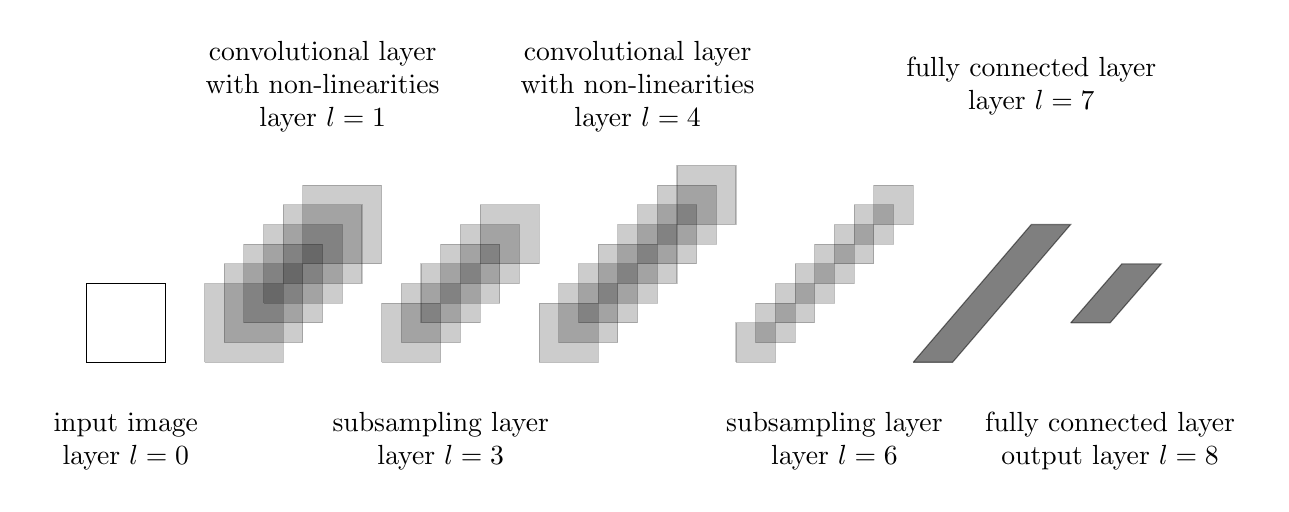
\begin{tikzpicture}
		\node at (0.5,-1){\begin{tabular}{c}input image\\layer $l = 0$\end{tabular}};
		
		\draw (0,0) -- (1,0) -- (1,1) -- (0,1) -- (0,0);
		
		\node at (3,3.5){\begin{tabular}{c}convolutional layer\\with non-linearities\\layer $l = 1$\end{tabular}};
		
		\draw[fill=black,opacity=0.2,draw=black] (2.75,1.25) -- (3.75,1.25) -- (3.75,2.25) -- (2.75,2.25) -- (2.75,1.25);
		\draw[fill=black,opacity=0.2,draw=black] (2.5,1) -- (3.5,1) -- (3.5,2) -- (2.5,2) -- (2.5,1);
		\draw[fill=black,opacity=0.2,draw=black] (2.25,0.75) -- (3.25,0.75) -- (3.25,1.75) -- (2.25,1.75) -- (2.25,0.75);
		\draw[fill=black,opacity=0.2,draw=black] (2,0.5) -- (3,0.5) -- (3,1.5) -- (2,1.5) -- (2,0.5);
		\draw[fill=black,opacity=0.2,draw=black] (1.75,0.25) -- (2.75,0.25) -- (2.75,1.25) -- (1.75,1.25) -- (1.75,0.25);
		\draw[fill=black,opacity=0.2,draw=black] (1.5,0) -- (2.5,0) -- (2.5,1) -- (1.5,1) -- (1.5,0);
		
		\node at (4.5,-1){\begin{tabular}{c}subsampling layer\\layer $l = 3$\end{tabular}};
		
		\draw[fill=black,opacity=0.2,draw=black] (5,1.25) -- (5.75,1.25) -- (5.75,2) -- (5,2) -- (5,1.25);
		\draw[fill=black,opacity=0.2,draw=black] (4.75,1) -- (5.5,1) -- (5.5,1.75) -- (4.75,1.75) -- (4.75,1);
		\draw[fill=black,opacity=0.2,draw=black] (4.5,0.75) -- (5.25,0.75) -- (5.25,1.5) -- (4.5,1.5) -- (4.5,0.75);
		\draw[fill=black,opacity=0.2,draw=black] (4.25,0.5) -- (5,0.5) -- (5,1.25) -- (4.25,1.25) -- (4.25,0.5);
		\draw[fill=black,opacity=0.2,draw=black] (4,0.25) -- (4.75,0.25) -- (4.75,1) -- (4,1) -- (4,0.25);
		\draw[fill=black,opacity=0.2,draw=black] (3.75,0) -- (4.5,0) -- (4.5,0.75) -- (3.75,0.75) -- (3.75,0);
		
		\node at (7,3.5){\begin{tabular}{c}convolutional layer\\with non-linearities\\layer $l = 4$\end{tabular}};
		
		\draw[fill=black,opacity=0.2,draw=black] (7.5,1.75) -- (8.25,1.75) -- (8.25,2.5) -- (7.5,2.5) -- (7.5,1.75);
		\draw[fill=black,opacity=0.2,draw=black] (7.25,1.5) -- (8,1.5) -- (8,2.25) -- (7.25,2.25) -- (7.25,1.5);
		\draw[fill=black,opacity=0.2,draw=black] (7,1.25) -- (7.75,1.25) -- (7.75,2) -- (7,2) -- (7,1.25);
		\draw[fill=black,opacity=0.2,draw=black] (6.75,1) -- (7.5,1) -- (7.5,1.75) -- (6.75,1.75) -- (6.75,1);
		\draw[fill=black,opacity=0.2,draw=black] (6.5,0.75) -- (7.25,0.75) -- (7.25,1.5) -- (6.5,1.5) -- (6.5,0.75);
		\draw[fill=black,opacity=0.2,draw=black] (6.25,0.5) -- (7,0.5) -- (7,1.25) -- (6.25,1.25) -- (6.25,0.5);
		\draw[fill=black,opacity=0.2,draw=black] (6,0.25) -- (6.75,0.25) -- (6.75,1) -- (6,1) -- (6,0.25);
		\draw[fill=black,opacity=0.2,draw=black] (5.75,0) -- (6.5,0) -- (6.5,0.75) -- (5.75,0.75) -- (5.75,0);
		
		\node at (9.5,-1){\begin{tabular}{c}subsampling layer\\layer $l = 6$\end{tabular}};
		
		\draw[fill=black,opacity=0.2,draw=black] (10,1.75) -- (10.5,1.75) -- (10.5,2.25) -- (10,2.25) -- (10,1.75);
		\draw[fill=black,opacity=0.2,draw=black] (9.75,1.5) -- (10.25,1.5) -- (10.25,2) -- (9.75,2) -- (9.75,1.5);
		\draw[fill=black,opacity=0.2,draw=black] (9.5,1.25) -- (10,1.25) -- (10,1.75) -- (9.5,1.75) -- (9.5,1.25);
		\draw[fill=black,opacity=0.2,draw=black] (9.25,1) -- (9.75,1) -- (9.75,1.5) -- (9.25,1.5) -- (9.25,1);
		\draw[fill=black,opacity=0.2,draw=black] (9,0.75) -- (9.5,0.75) -- (9.5,1.25) -- (9,1.25) -- (9,0.75);
		\draw[fill=black,opacity=0.2,draw=black] (8.75,0.5) -- (9.25,0.5) -- (9.25,1) -- (8.75,1) -- (8.75,0.5);
		\draw[fill=black,opacity=0.2,draw=black] (8.5,0.25) -- (9,0.25) -- (9,0.75) -- (8.5,0.75) -- (8.5,0.25);
		\draw[fill=black,opacity=0.2,draw=black] (8.25,0) -- (8.75,0) -- (8.75,0.5) -- (8.25,0.5) -- (8.25,0);
		
		\node at (12,3.5){\begin{tabular}{c}fully connected layer\\layer $l = 7$\end{tabular}};
		
		\draw[fill=black,draw=black,opacity=0.5] (10.5,0) -- (11,0) -- (12.5,1.75) -- (12,1.75) -- (10.5,0);
		
		\node at (13,-1){\begin{tabular}{c}fully connected layer\\output layer $l = 8$\end{tabular}};
		
		\draw[fill=black,draw=black,opacity=0.5] (12.5,0.5) -- (13,0.5) -- (13.65,1.25) -- (13.15,1.25) -- (12.5,0.5);
	\end{tikzpicture}
	\caption[Architecture of a traditional convolutional neural network.]{The architecture of the original convolutional neural network, as introduced in \cite{LeCunBoserDenkerHenderson:1989}, alternates between convolutional layers including hyperbolic tangent non-linearities and subsampling layers. In this illustration, the convolutional layers already include non-linearities and, thus, a convolutional layer actually represents two layers. The feature maps of the final subsampling layer are then fed into the actual classifier consisting of an arbitrary number of fully connected layers. The output layer usually uses softmax activation functions.}
	\label{fig:traditional-convolutional-network}
\end{figure}
We discuss both the traditional convolutional neural network as proposed in \cite{LeCunBoserDenkerHenderson:1989} as well as a modern variant as used in \cite{KrizhevskySutskeverHinton:2012}.

\subsubsection{Traditional Convolutional Neural Network}

In \cite{JarrettKavukcuogluRanzatoLeCun:2009}, the basic building block of traditional neural networks is $F_{\text{CSG}}$ -- $P_{\text{A}}$, while in \cite{LeCunBoserDenkerHenderson:1989}, the subsampling is accomplished within the convolutional layers and there are no gain coefficients used. In general, the unique characteristic of traditional convolutional neural networks lies in the hyperbolic tangent non-linearities and the weight sharing \cite{LeCunBoserDenkerHenderson:1989}. This is illustrated in figure \ref{fig:traditional-convolutional-network} where the non-linearities are included within the convolutional layers.

% The traditional convolutional neural network as introduced in \cite{LeCunBoserDenkerHenderson:1989} alternates between convolutional layer with included hyperbolic tangent non-linearities and a down-sampling layer to build up a feature hierarchy. The feature maps of the final subsampling layer are then used as input for the actual classifier consisting of one or multiple fully connected layers with softmax output activation. This basic architecture is illustrated in figure \ref{fig:traditional-convolutional-network}.

\subsubsection{Modern Convolutional Neural Networks}
\label{subsubsec:modern-convolutional-networks}

As example of a modern convolutional neural network we explore the architecture used in \cite{KrizhevskySutskeverHinton:2012} which gives excellent performance on the ImageNet Dataset \cite{ZeilerFergus:2013}. The architecture comprises five convolutional layers each followed by a rectified linear unit non-linearity layer, brightness normalization and overlapping pooling. Classification is done using three additional fully-connected layers. To avoid overfitting, \cite{KrizhevskySutskeverHinton:2012} uses dropout as regularization technique. Such a network can be specified by $F_{\text{CR}}$ -- $N_B$ -- $P$ where $F_{\text{CR}}$ denotes a convolutional layer followed by a non-linearity layer with rectified linear units. Details can be found in \cite{KrizhevskySutskeverHinton:2012}. 

In \cite{CiresanMeierSchmidhuber:2012} the authors combine several deep convolutional neural networks which have a similar architecture as described above and average their classification/prediction result. This architecture is referred to as multi-column deep convolutional neural network.

